\section{Random Stuff}

% Manually typeset a chapter quote
\vspace*{-2mm}
{\raggedleft \begin{minipage}{.3\textwidth}
	\footnotesize I never said half the shit people say I did.
	\\\rule{\textwidth}{0.35mm}\\
	\hspace*{\fill}\textit{Albert Einstein}
\end{minipage} \par}
\bigskip

% Line centered on page
\centerline{\mbox{\textsc{Welcome to \uline{this}. where typographical conventions are blasted to smithereens.}}}

% Plaster something over text using manual hacky space commands and also colors
\vspace*{-1.28cm}\hspace*{3.5cm}\scalebox{0.7}{\rotatebox{15}{\fboxrule0.35mm\fcolorbox[HTML]{DFDFDF}{F7F7F7}{\color[HTML]{702FFF}You're just nitpicking and biased, I win, bye bye \raisebox{.25ex}{\scalebox{0.75}{$\heartsuit$}}}}} % https://www.youtube.com/watch?v=sBqk7I5-0I0

\bigskip
\hrule
% Typeset a poem?...
\def\poemline<#1>{{#1}\\}%{\hspace*{1.5cm}{#1}\hspace*{\fill}\\}
\begin{figure}[H]
	\centering
	\sffamily
	\bfseries
	\color{textcol!90!pagecol}
	\poemline<suckity shillity why am i type>%
	\poemline<all of this bullshit that i have to write>%
	\poemline<i could have just copied some text from the web>%
	\poemline<lorem ipsum or whatever it says>%
\end{figure} % https://www.youtube.com/watch?v=1QYxJ69pY0E
\hrule
\bigskip

Recall how under canonical circumstances ($\rightarrow$ cit. \cite{PM10}) equation \big(\ref{eq:conjecture}\big) is believed to be provable from the axioms.
\begin{equation}
	\tag{4.2.1.1}
	\label{eq:conjecture}
	1 + 1 \approx{} 2
\end{equation}
Based.\ on this and making use of some simple re-indexing we have the following trivial result

\normalmarginpar\marginpar{
	\raggedright
	\textcolor{textcol!12.5!pagecol}{...what the \textsl{heeell}} \emoji{Walter}
}
% Demonstrate clusterfuck
\bigskip\resizebox{\textwidth}{!}{\begin{minipage}{2\textwidth}
	\protect{\begin{displaymath}
		\raisebox{0.3ex}{$l\kern-.14em q$}^\bullet(\Lambda)
		= \underbrace{e^{i\pi} + 1} _ {=\ 0}
		- \prod _ {i=0} ^ \infty
		\mleft[
			\operatornamewithlimits{arg\,ker} _ {
				\substack{
					r\in\R^\times \\
					\nexists n\,:\,r=F_n
				}
			}
			\bigcup _ {\ell\in\Lambda}
			\left\{
				\ell\circ\varphi_0\in\mathcal{C}^\infty
			\;\middle\vert\;
				\varphi_0
				\triangleq
				\operatornamewithlimits{
					\emoji{trollface}%\raisebox{-.8ex}{\includegraphics[height=16pt]{trollQ}}
				} _ {k=1} ^ {\infty}
				\zeta^{(r)}(k!!)
				\land
				\mleft(
					\liminf _ {\chi\to 0^-} \varphi_0(\chi) \notin\mathbb{Q}_{\geq0}
					\lor
					\mleft(
						\forall p\neq q :
							p \equiv_{251} \ceil{(\ell\cdot\digamma)(q)}
							\rightarrow
							\operatorname{supp}(\partial\varphi_0)=\varnothing
					\mright)
				\mright)
			\right\}
		\mright]
		+ \mleft.\frac{7\sqrt[\varepsilon]{\pi}}{12}\mright|^{\varepsilon=\sqrt2}
	\end{displaymath}}
\end{minipage}}

\bigskip
% Demonstrate unbreakable paragraphs - https://texfaq.org/FAQ-nopagebrk
\needspace{2\baselineskip}
\textit{\large\guillemotleft What are some of the “ugliest” parts of math?\guillemotright}
% Demonstrate list of descriptions with nice indents
\begin{description}[nosep,noitemsep,leftmargin=5mm]
	\item[Point-set topology.] Too many pathologies. Nowadays the only topologies for me are Grothendieck topologies.
	\item[Weights, in the context of Lie algebras.] The constructions are high\-ly non-ca\-no\-ni\-cal if not even arbitrary sometimes.
	\item[Elementary topoi.] Unless you're a logician, I can't see why you would prefer them to honest-to-Grothendieck sheaf topoi (feel free to change my mind).
	\item[Classical algebraic geometry à la Weil.] It was a mess (again, due to point-set topology being a pain), and not to mention very restrictive, as varieties only behave well over algebraically closed fields.
	\item[Topological vector spaces.] They are not ugly per se, but extremely delicate and subtle, and daing with them can sometimes involve hours if not days trying to find the right norm on a perfectly fine algebraic object (e.g. tensor products of Banach spaces).
	\item[Tate's rigid analytic varieties and Berkovich spaces.] They are practical and easy to visualise, but better to have a nice category with bad objects than a bad category of nice objects. One also needs to impose all sorts of extra finiteness conditions on them in order to be able to even begin computing their cohomologies. Luckily, these categories embed into the category of adic spaces (in the sense of Huber), which is much nicer, especially if you were to restrict down to the subcategory of perfectoid spaces.
\end{description}
% Demonstrate overlapping of symbols - https://tex.stackexchange.com/questions/620022/overlay-symbols-via-ooalign
(\^{} What the heck is \href{https://www.reddit.com/r/math/comments/rud9uq/comment/hr1mdli}{this} guy talking about) % https://www.reddit.com/r/math/comments/rud9uq/comment/hr1mdli

% Add frame directly onto content
%\frame{
%	\resizebox{0.95\textwidth}{!}{
%		The phrase "it's just a game" is such a weak mindset. You are ok with what happened, losing, imperfection of a craft. When you stop getting angry after losing, you've lost twice.
%	}
%}

%\bigskip
%\hrule
%\centerline{\resizebox{\textwidth}{!}{$\neg\exists x : \forall y : (P(y,x) \leftrightarrow \neg P(y,y))$}}
%\hrule

\newpage
\hfill$\underset{\textit{so below}}{\textit{as above}}$

\needspace{2\baselineskip}
\textit{\textbf{``What's your Sauce Code?''}}
\begingroup
	\makeatletter
		\DeclareRobustCommand\ttfamily{
			\not@math@alphabet\ttfamily\mathtt
			\fontfamily\ttdefault\footnotesize\selectfont
		}
	\makeatother % https://tex.stackexchange.com/questions/158778/all-ttfamily-font-change-font-size#158779
	\color{-pagecol}
% Demonstrate some unformatted code
\begin{listing}{1}
double a[4][4];
double b[4][4];
double c[4][4]; // set to zero
/* Multiply 4 x 4 matrices a and b */
void mmm(double *a, double *b, double *c, int n) {
  int i, j, k;
  for (i = 0; i < 4; i++)
    for (j = 0; j < 4; j++)
      for (k = 0; k < 4; k++)
        c[i*4+j] += a[i*4 + k]*b[k*4 + j];
}
// At this point, I'd like to take a moment to speak to you about the Adobe PSD
// format. PSD is not a good format. PSD is not even a bad format. Calling it
// such would be an insult to other bad formats, such as PCX or JPEG. No, PSD
// is an abysmal format. Having worked on this code for several weeks now, my
// hate for PSD has grown to a raging fire that burns with the fierce passion
// of a million suns.
//
// If there are two different ways of doing something, PSD will do both, in
// different places. It will then make up three more ways no sane human would
// think of, and do those too. PSD makes inconsistency an art form. Why, for
// instance, did it suddenly decide that *these* particular chunks should be
// aligned to four bytes, and that this alignement should *not* be included in
// the size? Other chunks in other places are either unaligned, or aligned with
// the alignment included in the size. Here, though, it is not included. Either
// one of these three behaviours would be fine. A sane format would pick one.
// PSD, of course, uses all three, and more.
//
// Trying to get data out of a PSD file is like trying to find something in the
// attic of your eccentric old uncle who died in a freak freshwater shark
// attack on his 58th birthday. That last detail may not be important for the
// purposes of the simile, but at this point I am spending a lot of time
// imagining amusing fates for the people responsible for this Rube Goldberg of
// a file format.
//
// Earlier, I tried to get a hold of the latest specs for the PSD file format.
// To do this, I had to apply to them for permission to apply to them to have
// them consider sending me this sacred tome. This would have involved faxing
// them a copy of some document or other, probably signed in blood. I can only
// imagine that they make this process so difficult because they are intensely
// ashamed of having created this abomination. I was naturally not gullible
// enough to go through with this procedure, but if I had done so, I would have
// printed out every single page of the spec, and set them all on fire. Were it
// within my power, I would gather every single copy of those specs, and launch
// them on a spaceship directly into the sun.
//
// PSD is not my favourite file format.\end{listing}
\endgroup % https://github.com/gco/xee/blob/master/XeePhotoshopLoader.m#L108-L136

\vfill\hfill$\underset{\textit{so above}}{\textit{as below}}$

%\clearpage
%\vspace*{\fill}
%\begin{figure}[H]
%	\raggedleft
%	\textit{\large ``In this world, is the destiny of mankind controlled by some transcendental entity or law? Is it like the hand of God hovering above? At least it is true that man has no control, even over his own will. Man takes up the sword in order to shield the small wound in his heart sustained in a far-off time beyond remembrance. Man wields the sword so that he may die smiling in some far-off time beyond perception.''}
%\end{figure}
%\vspace*{\fill}
%\clearpage

\clearpage
	\pagecolor{pergament}
	\color{sepia}
	\begin{multicols}{2}
% Demonstrate input file
	\raisebox{-0.4ex}{\huge V}\resizebox{0pt}{0pt}{on\space Franz\space Kafka\space -\space v}or dem Gesetz steht ein Türhüter. Zu diesem Türhüter kommt ein Mann vom Lande und bittet um Eintritt in das Gesetz. Aber der Türhüter sagt, dass er ihm jetzt den Eintritt nicht gewähren könne. Der Mann überlegt und fragt dann, ob er also später werde eintreten dürfen. „Es ist möglich,“ sagt der Türhüter, „jetzt aber nicht.“ Da das Tor zum Gesetz offen steht wie immer und der Türhüter beiseite tritt, bückt sich der Mann, um durch das Tor in das Innere zu sehen. Als der Türhüter das merkt, lacht er und sagt: „Wenn es dich so lockt, versuche es doch trotz meines Verbotes hineinzugehen. Merke aber: Ich bin mächtig. Und ich bin nur der unterste Türhüter. Von Saal zu Saal stehen aber Türhüter, einer mächtiger als der andere. Schon den Anblick des Dritten kann nicht einmal ich mehr ertragen.“ Solche Schwierigkeiten hat der Mann vom Lande nicht erwartet; das Gesetz soll doch jedem und immer zugänglich sein, denkt er, aber als er jetzt den Türhüter in seinem Pelzmantel genauer ansieht, seine grosse Spitznase, den langen, dünnen, schwarzen tartarischen Bart, entschliesst er sich doch lieber zu warten, bis er die Erlaubnis zum Eintritt bekommt. Der Türhüter gibt ihm einen Schemel und lässt ihn seitwärts von der Tür sich niedersetzen. Dort sitzt er Tage und Jahre. Er macht viele Versuche eingelassen zu werden und ermüdet den Türhüter durch seine Bitten. Der Türhüter stellt öfters kleine Verhöre mit ihm an, fragt ihn über seine Heimat aus und nach vielem andern, es sind aber teilnahmslose Fragen, wie sie grosse Herren stellen, und zum Schlusse sagt er ihm immer wieder, dass er ihn noch nicht einlassen könne. Der Mann, der sich für seine Reise mit vielem ausgerüstet hat, verwendet alles, und sei es noch so wertvoll, um den Türhüter zu bestechen. Dieser nimmt zwar alles an, aber sagt dabei: „Ich nehme es nur an, damit du nicht glaubst, etwas versäumt zu haben.“ Während der vielen Jahre beobachtet der Mann den Türhüter fast ununterbrochen. Er vergisst die andern Türhüter und dieser erste scheint ihm das einzige Hindernis für den Eintritt in das Gesetz. Er verflucht den unglücklichen Zufall, in den ersten Jahren rücksichtslos und laut, später als er alt wird, brummt er nur noch vor sich hin. Er wird kindisch und da er in dem jahrelangen Studium des Türhüters auch die Flöhe in seinem Pelzkragen erkannt hat, bittet er auch die Flöhe ihm zu helfen und den Türhüter umzustimmen. Schliesslich wird sein Augenlicht schwach und er weiss nicht, ob es um ihn wirklich dunkler wird oder ob ihn nur seine Augen täuschen. Wohl aber erkennt er jetzt im Dunkel einen Glanz, der unverlöschlich aus der Türe des Gesetzes bricht. Nun lebt er nicht mehr lange. Vor seinem Tode sammeln sich in seinem Kopfe alle Erfahrungen der ganzen Zeit zu einer Frage, die er bisher an den Türhüter noch nicht gestellt hat. Er winkt ihm zu, da er seinen erstarrenden Körper nicht mehr aufrichten kann. Der Türhüter muss sich tief zu ihm hinunterneigen, denn der Grössenunterschied hat sich sehr zu ungunsten des Mannes verändert. „Was willst du denn jetzt noch wissen?“ fragt der Türhüter, „du bist unersättlich.“ „Alle streben doch nach dem Gesetz,“ sagt der Mann, „wieso kommt es, dass in den vielen Jahren niemand ausser mir Einlass verlangt hat?“ Der Türhüter erkennt, dass der Mann schon an seinem Ende ist und, um sein vergehendes Gehör noch zu erreichen, brüllt er ihn an: „Hier konnte niemand sonst Einlass erhalten, denn dieser Eingang war nur für dich bestimmt. Ich gehe jetzt und schliesse ihn.“

	\end{multicols}
	\fancypagestyle{gesetzstyle}{
		\fancyhf{} \renewcommand{\headrulewidth}{0pt}
		\fancyhead[C]{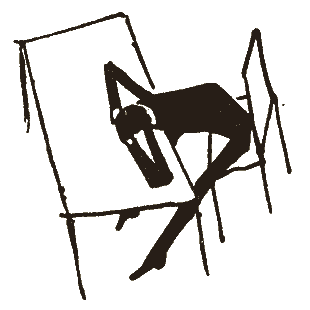
\includegraphics[height=20pt]{kafka}}
	}\thispagestyle{gesetzstyle}
	\color{textcol}
	\afterpage{\nopagecolor}
\clearpage